\documentclass[11pt]{beamer}

% Theme
\usetheme{Madrid}
\usecolortheme{default}

% Packages
\usepackage{amsmath,amssymb,amsthm}
\usepackage{mathtools}
\usepackage{listings}
\usepackage{xcolor}
\usepackage{tikz}
\usepackage{stmaryrd}
\usepackage{syntax}
\usepackage{bussproofs}
\usepackage{hyperref}
\usetikzlibrary{positioning, arrows.meta}


% Hoare Logic Commands
\renewcommand{\hoare}[3]{\{#1\}\; #2\; \{#3\}}
\newcommand{\assert}[1]{\{#1\}}
\newcommand{\pre}[1]{\{#1\}}
\newcommand{\post}[1]{\{#1\}}
\newcommand{\inv}[1]{\{#1\}}
\newcommand{\wlp}{\mathit{wlp}}
\renewcommand{\wp}{\mathit{wp}} % Changed from \newcommand
\renewcommand{\sp}{\mathit{sp}} % Changed from \newcommand
\renewcommand{\skip}{\texttt{skip}} % Changed from \newcommand
\newcommand{\assign}[2]{#1 := #2}
\newcommand{\seq}[2]{#1;\, #2}
\newcommand{\ifte}[3]{\texttt{if } #1 \texttt{ then } #2 \texttt{ else } #3}
\newcommand{\while}[2]{\texttt{while } #1 \texttt{ do } #2}
\renewcommand{\implies}{\Rightarrow} % Changed from \newcommand
\newcommand{\subst}[3]{#1[#2/#3]}
\newcommand{\bnfdef}{\mathrel{::=}}
\newcommand{\bnfor}{\;\mid\;}

% Code listing settings
\lstset{
    basicstyle=\ttfamily\footnotesize,
    keywordstyle=\color{blue}\bfseries,
    commentstyle=\color{green!60!black},
    stringstyle=\color{red},
    showstringspaces=false,
    numbers=left,
    numberstyle=\tiny\color{gray},
    stepnumber=1,
    numbersep=5pt,
    backgroundcolor=\color{gray!10},
    frame=single,
    frameround=tttt,
    framesep=5pt,
    breaklines=true,
    tabsize=2,
    captionpos=b,
    morekeywords={assert, assume, invariant, requires, ensures, modifies},
    escapeinside={(*}{*)},
}

% Define languages
\lstdefinelanguage{pseudocode}{
    keywords={if, then, else, while, do, for, to, skip, assert, assume, invariant},
    morecomment=[l]{//},
    morecomment=[s]{/*}{*/},
}

% Title
\title{Hoare Logic}
\subtitle{Program Verification}
\author{Your Name}
\date{\today}

\begin{document}

\begin{frame}
    \titlepage
\end{frame}

\begin{frame}{Outline}
    \tableofcontents
\end{frame}

\section{A Little Programming Language}

\begin{frame}{Syntax of the Language}
    \framesubtitle{Based on Backus-Naur Form (BNF)}

    \colorbox{yellow}{\bfseries Expressions:}
    \[ E \bnfdef N \bnfor V \bnfor E_1 + E_2 \bnfor E_1 - E_2 \bnfor E_1 \times E_2 \bnfor \dots \]

    \vspace{0.7cm}

    \colorbox{yellow}{\bfseries Boolean expressions:}
    \[ B \bnfdef \mathbf{T} \bnfor \mathbf{F} \bnfor E_1=E_2 \bnfor E_1 \le E_2 \bnfor \dots \]

    \vspace{0.7cm}

    \colorbox{yellow}{\bfseries Commands:}
    \[
        \begin{array}{lcl}
            C & \bnfdef & \assign{V}{E} \\
            & \bnfor  & \seq{C_1}{C_2} \\
            & \bnfor  & \text{IF } B \text{ THEN } C_1 \text{ ELSE } C_2 \\
            & \bnfor  & \text{WHILE } B \text{ DO } C'
        \end{array}
    \]
\end{frame}

\begin{frame}[fragile]{Example Programs - 1}
    \framesubtitle{Illustrating the language syntax}

    \begin{block}{Factorial of a number `n`}
        This program computes $n!$ and stores the result in the variable `fact`. It assumes the variable `n` holds a non-negative integer. The body of the `while` loop is a sequence of two assignment commands.
        \begin{lstlisting}[language=pseudocode, numbers=none]
fact := 1;
i := n;
while i > 0 do
    fact := fact * i;
    i := i - 1
        \end{lstlisting}
    \end{block}

    \end{frame}
\begin{frame}[fragile]{Example Programs - 2}


    \begin{block}{Maximum of two numbers `x` and `y`}
        This program uses a conditional statement to find the maximum of two numbers, `x` and `y`, and stores the result in `max`.
        \begin{lstlisting}[language=pseudocode, numbers=none]
if x <= y then
    max := y
else
    max := x
        \end{lstlisting}
    \end{block}
\end{frame}


% Section 1.5: Introduction to Hoare's Notation
\section{Hoare's Notation}

\begin{frame}{Hoare's Notation}
    \begin{block}{Historical Context}
        C.A.R. Hoare introduced the following notation called a \textbf{partial correctness specification} for specifying what a program does:
        \begin{center}
            \Large $\hoare{P}{C}{Q}$
        \end{center}
    \end{block}
    
    \begin{block}{Components}
        \begin{itemize}
            \item $C$ is a command (a program or program fragment)
            \item $P$ and $Q$ are conditions on the program variables used in $C$
            \item $P$ is called the \textbf{precondition}
            \item $Q$ is called the \textbf{postcondition}
        \end{itemize}
    \end{block}
\end{frame}

\begin{frame}{Writing Conditions}
    \begin{block}{Mathematical Notation}
        Conditions on program variables will be written using standard mathematical notations together with \textbf{logical operators}:
        \begin{itemize}
            \item $\wedge$ (and)
            \item $\vee$ (or)
            \item $\neg$ (not)
            \item $\Rightarrow$ (implies)
        \end{itemize}
    \end{block}
    
    \begin{example}
        Some example conditions:
        \begin{itemize}
            \item $x > 0 \wedge y \geq 0$ (x is positive AND y is non-negative)
            \item $x = 0 \vee y = 0$ (x equals zero OR y equals zero)
            \item $x > 0 \Rightarrow x^2 > 0$ (if x is positive, then x squared is positive)
        \end{itemize}
    \end{example}
\end{frame}

\begin{frame}{Evolution of Notation}
    \begin{block}{Historical Note}
        Hoare's original notation was $P\ \{C\}\ Q$ not $\hoare{P}{C}{Q}$, but the latter form is now more widely used.
    \end{block}
    
    \begin{block}{Alternative Notations}
        You may encounter different notations in the literature:
        \begin{itemize}
            \item Original: $P\ \{C\}\ Q$
            \item Modern: $\hoare{P}{C}{Q}$
            \item Some texts: $\{P\}\ C\ \{Q\}$ (without special formatting)
        \end{itemize}
        All represent the same concept: a partial correctness specification.
    \end{block}
\end{frame}

\begin{frame}{Partial Correctness}
    \begin{block}{What is Partial Correctness?}
        A Hoare triple $\hoare{P}{C}{Q}$ expresses \textbf{partial correctness}:
        \begin{quote}
            \emph{If} the precondition $P$ is true before executing command $C$, \emph{and if} $C$ terminates, \emph{then} the postcondition $Q$ will be true after execution.
        \end{quote}
    \end{block}
    
    \begin{alertblock}{Important: Termination Not Guaranteed}
        Partial correctness does \textbf{not} guarantee that the program terminates!
        \begin{itemize}
            \item It only says what must be true \emph{if} the program terminates
            \item A program that loops forever can still be partially correct
            \item Total correctness = Partial correctness + Termination
        \end{itemize}
    \end{alertblock}
\end{frame}

\begin{frame}{Reading Hoare Triples}
    \begin{block}{How to Read $\hoare{P}{C}{Q}$}
        The triple $\hoare{P}{C}{Q}$ can be read as:
        \begin{enumerate}
            \item ``If $P$ is true, then after $C$ executes, $Q$ will be true''
            \item ``$C$ transforms states satisfying $P$ into states satisfying $Q$''
            \item ``Starting from $P$, command $C$ establishes $Q$''
        \end{enumerate}
    \end{block}
    
    \begin{example}[Simple Assignment]
        $\hoare{x = 5}{\assign{y}{x + 1}}{y = 6}$
        
        This reads as: ``If $x$ equals 5 before the assignment, then $y$ will equal 6 after the assignment.''
    \end{example}
\end{frame}

\begin{frame}{Meaning of Hoare's Notation}
    \begin{block}{Formal Definition}
        $\hoare{P}{C}{Q}$ is true if:
        \begin{itemize}
            \item whenever $C$ is executed in a state satisfying $P$
            \item and \emph{if} the execution of $C$ terminates
            \item then the state in which $C$ terminates satisfies $Q$
        \end{itemize}
    \end{block}
    
    \begin{example}[Assignment Command]
        Consider: $\hoare{X = 1}{X := X + 1}{X = 2}$
        \begin{itemize}
            \item $P$ is the condition that the value of X is 1
            \item $Q$ is the condition that the value of X is 2
            \item $C$ is the assignment command $X := X + 1$ (i.e. `X becomes X+1')
        \end{itemize}
    \end{example}
\end{frame}

\begin{frame}{Truth and Falsity of Hoare Triples}
    \begin{example}[True Triple]
        $\hoare{X = 1}{X := X + 1}{X = 2}$ is \textbf{true}
        
        \textbf{Why?} Starting from a state where $X = 1$, executing $X := X + 1$ results in $X = 2$.
    \end{example}
    
    \begin{example}[False Triple]
        $\hoare{X = 1}{X := X + 1}{X = 3}$ is \textbf{false}
        
        \textbf{Why?} Starting from $X = 1$, executing $X := X + 1$ results in $X = 2$, not $X = 3$.
    \end{example}
    
    \begin{alertblock}{Key Insight}
        A Hoare triple is a mathematical statement that can be either true or false. It makes a claim about what happens when a program executes.
    \end{alertblock}
\end{frame}

\begin{frame}{Hoare Logic and Verification Conditions}
    \begin{block}{What is Hoare Logic?}
        Hoare Logic is a \textbf{deductive proof system} for Hoare triples $\hoare{P}{C}{Q}$
        \begin{itemize}
            \item Provides axioms and inference rules for proving program correctness
            \item Forms the theoretical foundation for program verification
        \end{itemize}
    \end{block}
    
    \begin{block}{Direct Verification with Hoare Logic}
        \textbf{Advantages:}
        \begin{itemize}
            \item Original proposal by Hoare
            \item Provides complete formal proofs
        \end{itemize}
        
        \textbf{Disadvantages:}
        \begin{itemize}
            \item Tedious and error-prone for humans
            \item Impractical for large programs
            \item Requires detailed manual proof construction
        \end{itemize}
    \end{block}
\end{frame}

\begin{frame}{Verification Conditions}
    \begin{block}{Modern Approach: Verification Conditions}
        Can `compile' proving $\hoare{P}{C}{Q}$ to \textbf{verification conditions}
        \begin{itemize}
            \item More natural for automated reasoning
            \item Basis for computer-assisted verification
            \item Separates program logic from mathematical reasoning
        \end{itemize}
    \end{block}
    
    \begin{block}{Key Property}
        Proof of verification conditions is \textbf{equivalent} to proof with Hoare Logic
        \begin{itemize}
            \item Hoare Logic can be used to \emph{explain} verification conditions
            \item Both approaches prove the same correctness properties
            \item Verification conditions are more amenable to automation
        \end{itemize}
    \end{block}
    
    \begin{example}[Simple Verification Condition]
        To prove $\hoare{x > 0}{y := x + 1}{y > 1}$, we generate the verification condition:
        \[x > 0 \Rightarrow (x + 1) > 1\]
        This is a pure mathematical statement that can be proved without considering program execution.
    \end{example}
\end{frame}
\begin{frame}{What is a Program Specification?}
    \begin{block}{The Contract}
        A program specification acts as a formal contract. It precisely describes the expected behavior of a piece of code.
        \begin{itemize}
            \item It does \textbf{not} describe \emph{how} the program works.
            \item It \textbf{does} describe \emph{what} the program must accomplish.
        \end{itemize}
    \end{block}
    \begin{block}{Key Components}
        A specification consists of two main parts:
        \begin{itemize}
            \item \textbf{Precondition:} A condition that must be true \emph{before} the program is executed.
            \item \textbf{Postcondition:} A condition that is guaranteed to be true \emph{after} the program terminates.
        \end{itemize}
    \end{block}
\end{frame}

\begin{frame}{Visualizing a Specification}
    \framesubtitle{From Initial to Final State}
    \begin{center}
        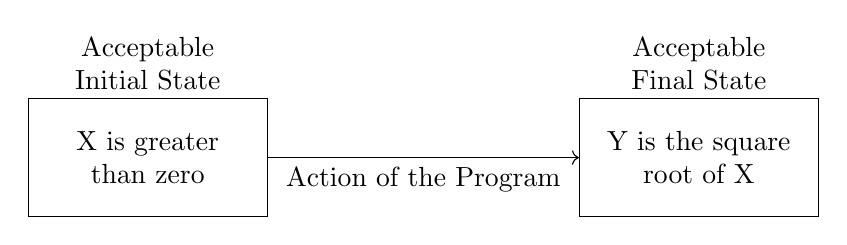
\begin{tikzpicture}
            % Define style for the boxes
            \tikzstyle{statebox} = [draw, rectangle, minimum height=1.5cm, text width=2.8cm, align=center]

            % Nodes for states
            \node [statebox] (initial) at (-1,0) {X is greater than zero};
            \node [statebox] (final) at (6,0) {Y is the square root of X};

            % Labels above the states
            \node [align=center] at (-1,1.2) {Acceptable \\ Initial State};
            \node [align=center] at (6,1.2) {Acceptable \\ Final State};

            % Arrow with label for the program's action
            \draw [->] (initial) -- node[below, align=center] {Action of the Program} (final);
        \end{tikzpicture}
    \end{center}
\end{frame}

\begin{frame}{The Precondition (P)}
    \begin{block}{Acceptable Initial State}
        The \textbf{precondition} defines the set of initial states for which the program is guaranteed to work correctly.
        \begin{itemize}
            \item It's an assumption about the values of program variables before execution.
            \item If the precondition is not met, the program has no obligations. It can crash, loop forever, or produce a wrong answer.
            \item Note: Reasoning about memory layout and heap requires \emph{Separation Logic}, an extension of Hoare Logic.
        \end{itemize}
    \end{block}
\end{frame}
\begin{frame}{The Precondition (P) - Example}


    \begin{example}
        For a program that calculates the square root of X, the informal precondition is:
        \begin{center}
            ``X is greater than zero''
        \end{center}
        The formal precondition, which we denote as $P$, is:
        \begin{center}
            $\pre{X > 0}$
        \end{center}
    \end{example}
\end{frame}

\begin{frame}{The Postcondition (Q)}
    \begin{block}{Acceptable Final State}
        The \textbf{postcondition} describes the state of the program after it has finished executing.
        \begin{itemize}
            \item It's the "promise" or "guarantee" of the specification.
            \item It typically relates the final values of variables to their initial values.
        \end{itemize}
    \end{block}
\end{frame}
\begin{frame}{The Postcondition (Q) - Example}
    \begin{example}
        For the square root program, the informal postcondition is:
        \begin{center}
            ``Y is the square root of X''
        \end{center}
        The formal postcondition, denoted as $Q$, is:
        \begin{center}
            $\post{Y \times Y = X \wedge Y \ge 0}$
        \end{center}
        (Note: we relate the final value of Y to the initial value of X).
    \end{example}
\end{frame}

\begin{frame}{Formal Specification: The Hoare Triple}
    \begin{block}{Combining Pre- and Postconditions}
        Hoare Logic provides a formal notation to write specifications, called a \textbf{Hoare Triple}.
        \[ \hoare{P}{S}{Q} \]
        This is read as:
        \begin{quote}
            If the precondition $P$ is true before executing the program $S$, and if $S$ terminates, then the postcondition $Q$ will be true afterward.
        \end{quote}
    \end{block}

    \begin{example}[Square Root Specification]
        Combining our previous examples, the specification for a square root program $S$ is:
        \[ \hoare{X > 0}{S}{Y \times Y = X \wedge Y \ge 0} \]
        Here, $S$ is the placeholder for the actual program code (the "Action").
    \end{example}
\end{frame}

\section{Boilerplate}
\begin{frame}{Hoare Triples}
    \begin{definition}[Hoare Triple]
        A \emph{Hoare triple} $\hoare{P}{S}{Q}$ consists of:
        \begin{itemize}
            \item Precondition $P$
            \item Program $S$
            \item Postcondition $Q$
        \end{itemize}
    \end{definition}
    
    \begin{block}{Meaning}
        If $P$ holds before executing $S$, and $S$ terminates, then $Q$ holds after execution.
    \end{block}
    
    \begin{example}
        $\hoare{x = 5}{\assign{y}{x + 1}}{y = 6}$
    \end{example}
\end{frame}

\begin{frame}[fragile]{Assignment Rule}
    \begin{block}{Assignment Axiom}
        \[
        \frac{}{\hoare{\subst{Q}{e}{x}}{\assign{x}{e}}{Q}}
        \]
    \end{block}
    
    \begin{example}
        To prove $\hoare{y = 5}{\assign{x}{y + 1}}{x = 6}$:
        \begin{itemize}
            \item $Q = (x = 6)$
            \item $e = y + 1$
            \item $\subst{Q}{e}{x} = (y + 1 = 6) \equiv (y = 5)$
        \end{itemize}
    \end{example}
\end{frame}

\begin{frame}[fragile]{Code Example}
    \begin{lstlisting}[language=pseudocode]
// (*$\pre{x \geq 0}$*)
y := 0;
z := 0;
while (y < x) do
    // (*$\inv{z = y \wedge y \leq x}$*)
    z := z + 1;
    y := y + 1;
// (*$\post{z = x}$*)
    \end{lstlisting}
\end{frame}

\begin{frame}{Inference Rules}
    \begin{columns}
        \column{0.5\textwidth}
        \begin{block}{Sequence Rule}
            \[
            \frac{\hoare{P}{S_1}{R} \quad \hoare{R}{S_2}{Q}}
                 {\hoare{P}{\seq{S_1}{S_2}}{Q}}
            \]
        \end{block}
        
        \column{0.5\textwidth}
        \begin{block}{Consequence Rule}
            \[
            \frac{P' \implies P \quad \hoare{P}{S}{Q} \quad Q \implies Q'}
                 {\hoare{P'}{S}{Q'}}
            \]
        \end{block}
    \end{columns}
\end{frame}

\begin{frame}{While Rule}
    \begin{block}{While Loop Rule}
        \[
        \frac{\hoare{I \wedge B}{S}{I}}
             {\hoare{I}{\while{B}{S}}{I \wedge \neg B}}
        \]
        where $I$ is the loop invariant.
    \end{block}
    
    \begin{example}
        For factorial computation:
        \begin{itemize}
            \item Invariant: $I = (f = n! / k!)$
            \item Guard: $B = (k > 0)$
            \item Body maintains invariant
        \end{itemize}
    \end{example}
\end{frame}

\begin{frame}[fragile]{Weakest Precondition Example}
    \begin{columns}
        \column{0.5\textwidth}
        \begin{block}{Program}
            \begin{lstlisting}[language=pseudocode,numbers=none]
x := x + 1;
y := x * 2;
            \end{lstlisting}
        \end{block}
        
        \column{0.5\textwidth}
        \begin{block}{Calculation}
            \begin{align*}
                \wp(\text{prog}, y > 10) &= \\
                \wp(x := x + 1, \wp(y := x * 2, y > 10)) &= \\
                \wp(x := x + 1, x * 2 > 10) &= \\
                \wp(x := x + 1, x > 5) &= \\
                x + 1 > 5 &= \\
                x > 4
            \end{align*}
        \end{block}
    \end{columns}
\end{frame}

\begin{frame}{Proof Tree Example}
    \begin{center}
    \begin{prooftree}
        \AxiomC{$\vdash \{x = 5\} \assign{y}{x} \{y = 5\}$}
        \AxiomC{$\vdash \{y = 5\} \assign{z}{y + 1} \{z = 6\}$}
        \BinaryInfC{$\vdash \{x = 5\} \assign{y}{x}; \assign{z}{y + 1} \{z = 6\}$}
    \end{prooftree}
    \end{center}
\end{frame}

\section{Advanced Topics}

\begin{frame}{Total Correctness}
    \begin{itemize}
        \item Partial correctness: $\hoare{P}{S}{Q}$
        \item Total correctness: $[P]\,S\,[Q]$
        \begin{itemize}
            \item Additionally guarantees termination
        \end{itemize}
    \end{itemize}
    
    \begin{block}{Variant Function}
        For while loops, need decreasing variant:
        \begin{itemize}
            \item $v \geq 0$ in loop body
            \item $v$ decreases each iteration
        \end{itemize}
    \end{block}
\end{frame}

\begin{frame}[fragile]{C Code Example}
    \begin{lstlisting}[language=C]
/*@ requires n >= 0;
    ensures \result == n * (n + 1) / 2;
@*/
int sum(int n) {
    int s = 0;
    int i = 0;
    /*@ loop invariant s == i * (i + 1) / 2;
        loop invariant 0 <= i <= n;
        loop variant n - i;
    @*/
    while (i < n) {
        i = i + 1;
        s = s + i;
    }
    return s;
}
    \end{lstlisting}
\end{frame}

\end{document}